\section*{Parte 5}

En esta parte se estudió que sucede al medir un tren de deltas y un tren de sinc en el analizador de espectros. La primera gran observación es que en la vida real no existe manera de producir una delta perfecta. Por tal motivo, la mejor manera de simular una delta es usar un tren de pulsos configurando el edge time y pulse with con el valor mínimo posible. 

Puesto a que el analizador de espectro muestra la señal de entrada en el dominio de la frecuencia, en este caso se debería observar los siguientes resultados:\par

Para el caso del tren de pulsos:

\begin{equation*}
 x(t)=\sum \Pi (\frac{t-nT}{\tau})
\end{equation*}

Luego la transformada de fourier es:

\begin{equation*}
X(f) = \sum_{k} AD \cdot sinc(kD) \delta(f-kf)
\end{equation*}

Luego para el caso del tren de sinc:

\begin{equation*}
x(t)=A\sum_{n=-\infty}^{\infty}
sinc\left(f_s\left(t-\frac{n}{f_0}\right)\right)
\end{equation*}

Luego la transformada de fourier es 

\begin{equation*}
X(f)=\sum_{k=-\infty}^{\infty}
\frac{A}{T}\,
\operatorname{rect}\left(\frac{k}{T}\right)
\delta\left(f-\frac{k}{T}\right)
\end{equation*}

\begin{figure}[h!]
    \centering

    \begin{minipage}[b]{0.45\textwidth}
        \centering
        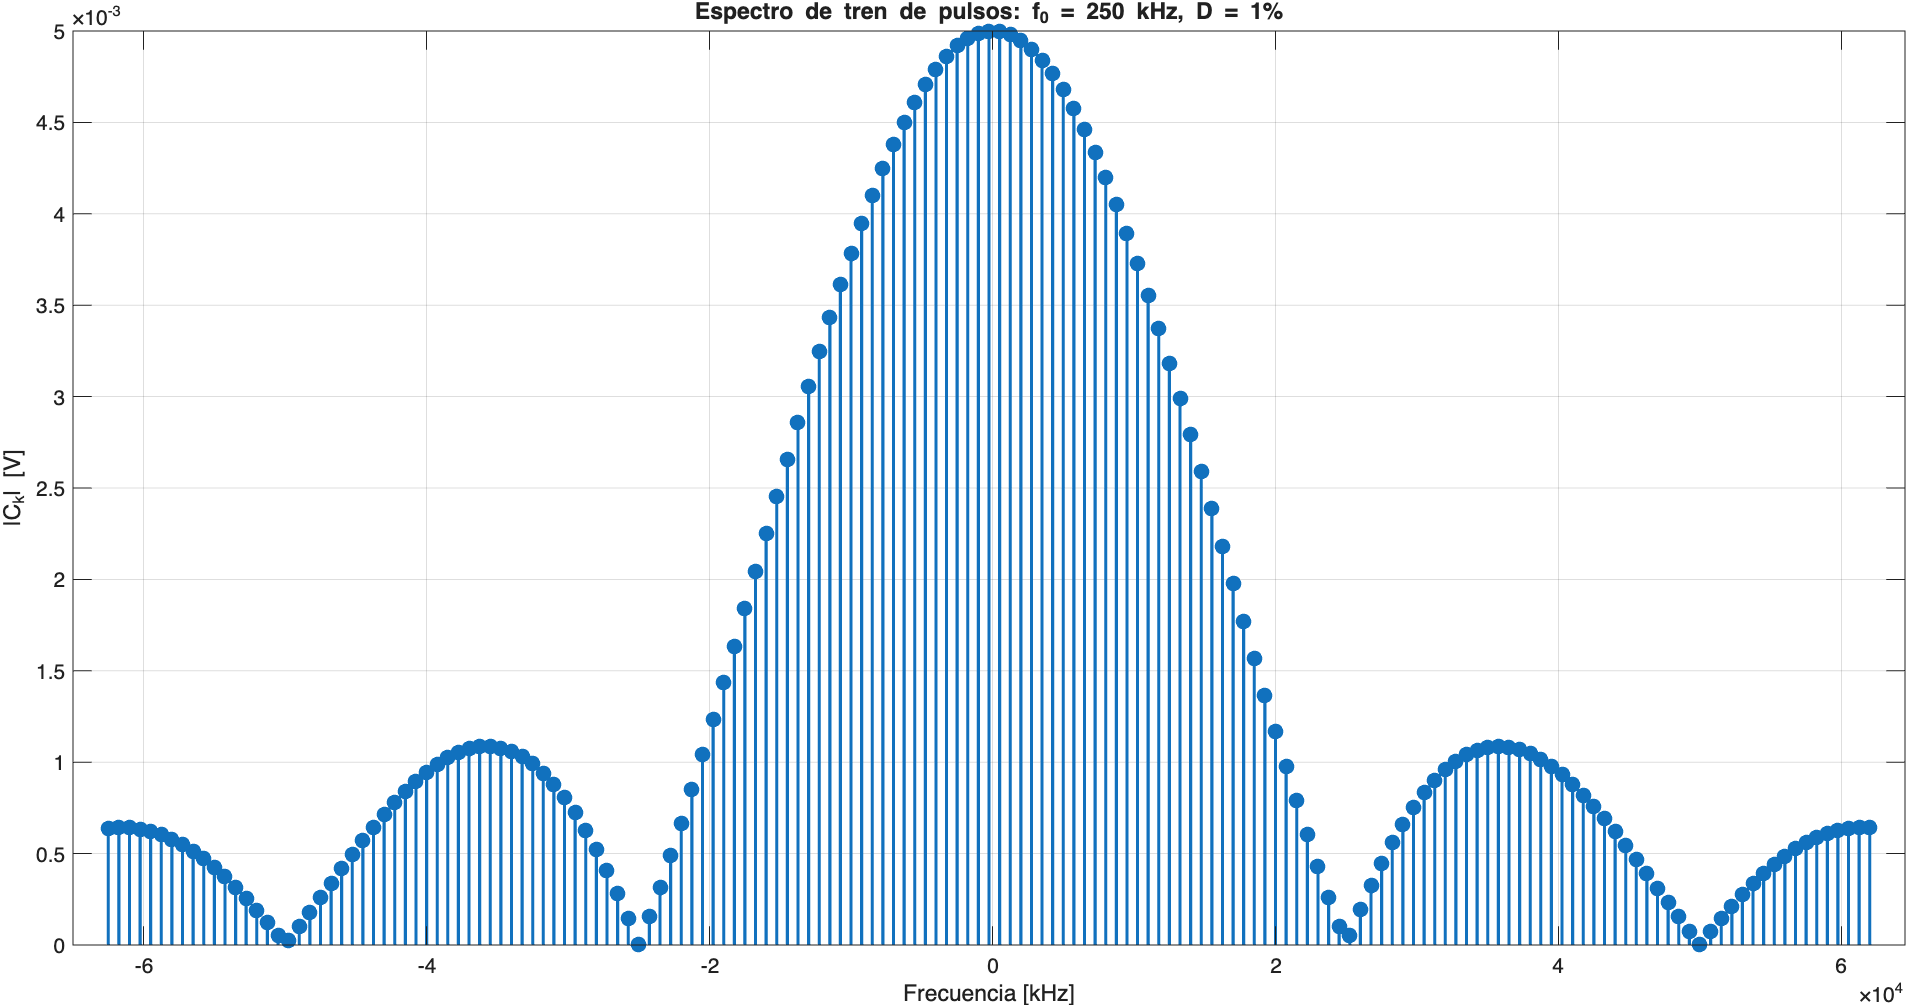
\includegraphics[width=\linewidth]
        {FOTOS_TP6/simulaciones/TFpulso.png}
        \caption{Simulación en Matlab de la transfromada de un tren de pulsos}
        \label{fig:matlabTFpulso}
    \end{minipage}
    \hfill
    \begin{minipage}[b]{0.45\textwidth}
        \centering
        
\includegraphics[width=0.75\linewidth
        ]{FOTOS_TP6/PARTE 5/pulso/p1/IMG_8334.jpeg}
        \caption{Foto del analizador de espectro}
        \label{fig:analizadorpulso}
    \end{minipage}

\end{figure}

\begin{figure}[H]
    \centering
    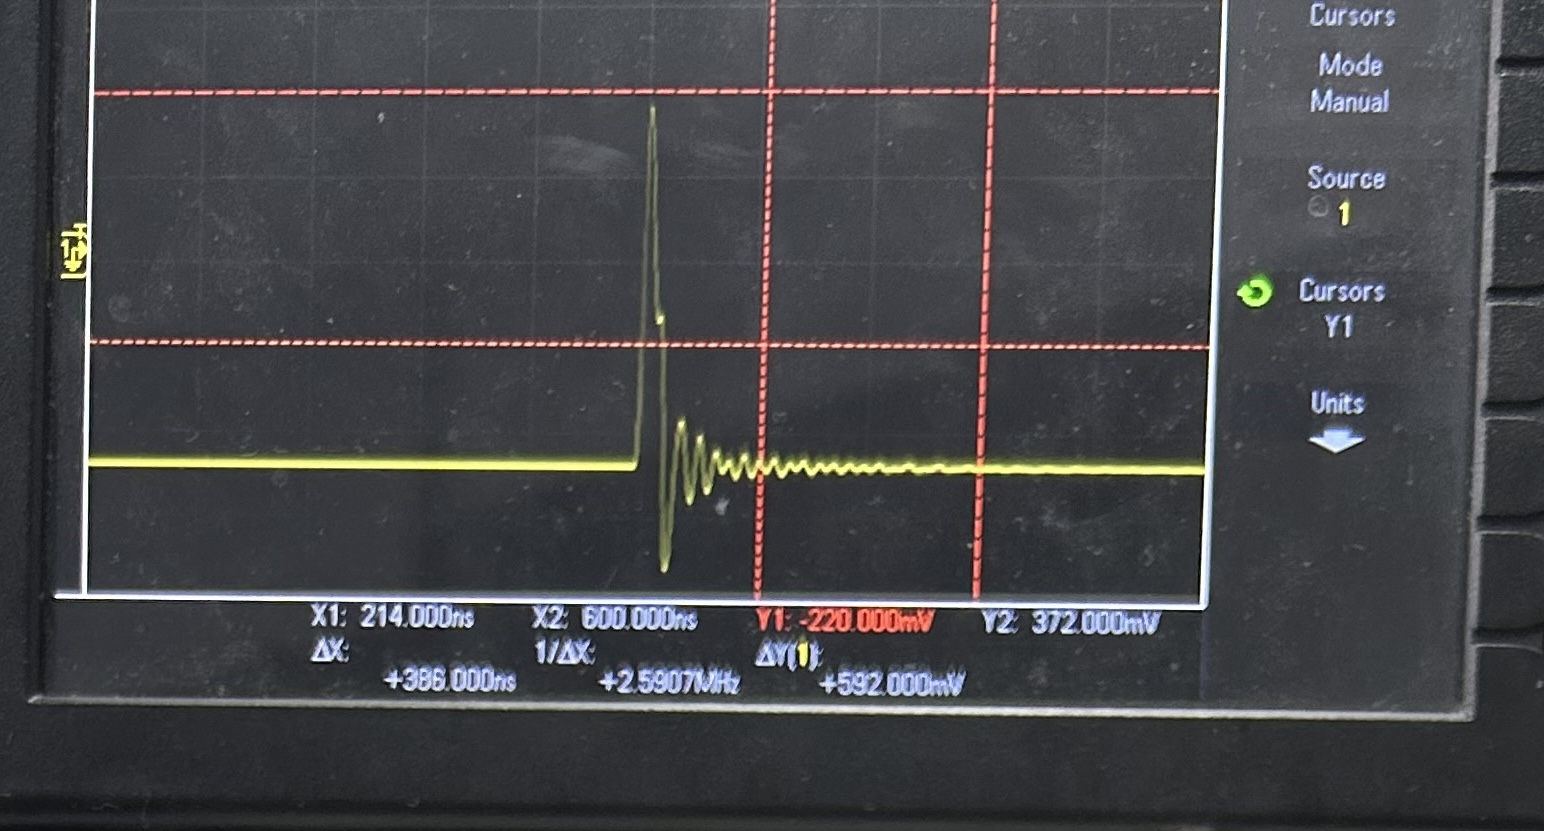
\includegraphics[width=0.8\textwidth]{FOTOS_TP6/PARTE 5/pulso/p1/pulso.jpeg}
    \caption{Pulso utilizado}
    \label{fig:pulso}
\end{figure}


En primer lugar, se simuló un tren de deltas con pulso with de $40ns$ y edge time de $8,4ns$ con frecuencia de $250kHz$. De esta manera se consigue un pulso con un D= 1\%. Al observar la figuras \ref{fig:matlabTFpulso} y \ref{fig:analizadorpulso}, se observó que los dos primeros ceros de la función coincidían en $25MHz$.\par

Por otra parte, en la Figura \ref{fig:pulso} puede observarse que la señal introducida al analizador de espectro mediante un tren de pulsos no se comporta idealmente como una suma de deltas. Esto se evidencia al observar la presencia de transitorios al final de la señal, los cuales introducen componentes adicionales e interferencias externas. No obstante, a pesar de estas limitaciones experimentales, se aprecia que la representación teórica del espectro de un tren de pulsos aproxima adecuadamente el comportamiento observado en el analizador de espectro.\par


En segundo lugar se simuló el caso de la señal compuesta por un tren de sinc. En este caso, hay que observar que existe una frecuencia $f_s$ que es la frecuencia interna del sinc y luego $f$ que es la frecuencia a la que los sinc se repiten. Para este análisis se configuró $f =250kH$ y luego se midió con el osciloscopio $f_s = 5MHz$, la cual venía predeterminada por el generador DIGILENT 33220A.\par

Con estos parámetros, se simuló en Matlab la transformada de la señal. Observar la figura \ref{fig:matlabTFsinc}. Luego al comparar con lo visto en el analizador de espectros se observó una buena concordancia con la simulación teórica. En particular se observa que en ambas figuras \ref{fig:matlabTFsinc} y \ref{fig:analizadorsinc}, el espectro estuvo conformado por un tren de deltas que terminaba a la misma frecuencia aproximada de $5MHz$. \par
No obstante una de las mayores diferencias que se observa es que la envolvente del tren de deltas observado teóricamente es un pulso perfecto, mientras que el observado en el analizador de espectros no lo es. Dos de los principales efectos que pueden explicar esto son el ancho de banda finito del generador y la duración de tiempo finita de la función sinc generada. En particular, estos efectos suelen manifestarse en las componentes de mayor frecuencia, las cuales, en este caso, se encuentran ubicadas en los extremos del espectro.


\begin{figure}[h!]
    \centering

    \begin{minipage}[b]{0.45\textwidth}
        \centering
        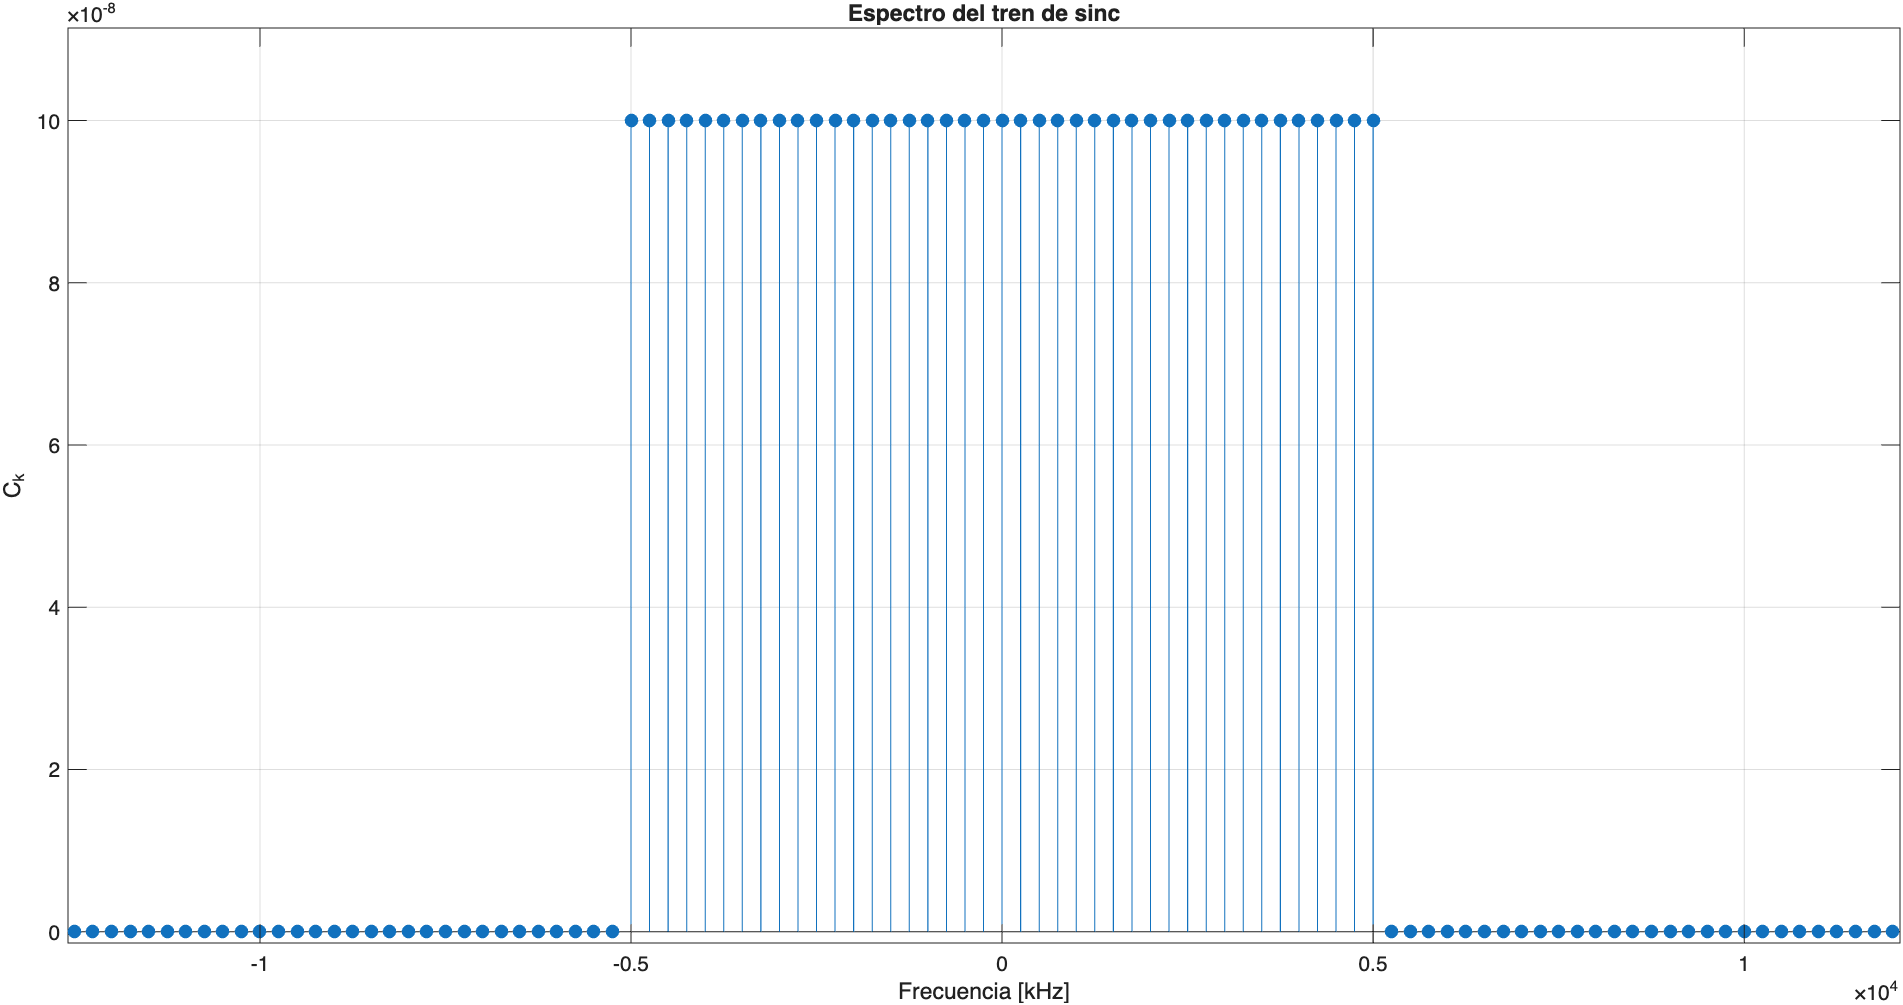
\includegraphics[width=\linewidth]
        {FOTOS_TP6/simulaciones/TFsinc.png}
        \caption{Simulación en Matlab de la transformada de un tren de sinc}
        \label{fig:matlabTFsinc}
    \end{minipage}
    \hfill
    \begin{minipage}[b]{0.45\textwidth}
        \centering
        
\includegraphics[width=0.75\linewidth
        ]{FOTOS_TP6/PARTE 5/sinc/IMG_8356.jpeg}
        \caption{Salida del analizador de espectro al introducir un tren de sinc}
        \label{fig:analizadorsinc}
    \end{minipage}

\end{figure}









